\documentclass{standalone}
\usepackage{tikz}
\usepackage{amsmath}

\begin{document}

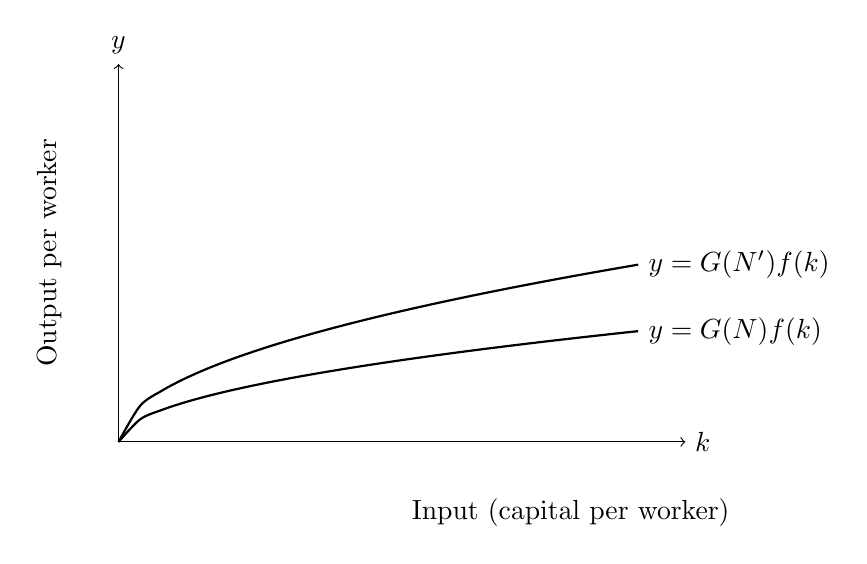
\begin{tikzpicture}[scale=1.2]

% Axes
\draw[->] (0,0) -- (6,0) node[right] {$k$};
\draw[->] (0,0) -- (0,4) node[above] {$y$};

% Labels
\node[below left] at (0,0) {};
\node[below right, align=center] at (3,-0.5) {Input (capital per worker)};
\node[rotate=90, above] at (-0.5,2) {Output per worker};

% Curves
\draw[thick, domain=0:5.5, smooth, variable=\x] plot ({\x},{0.5*sqrt(\x)}) node[right] {$y = G(N)f(k)$};
\draw[thick, domain=0:5.5, smooth, variable=\x] plot ({\x},{0.8*sqrt(\x)}) node[right] {$y = G(N')f(k)$};

\end{tikzpicture}

\end{document}